% =====================================================================
%  Data Mining · SGH · SMMD-ADA   —   Block 6 slide deck
%  Template: Frankfurt + seahorse + miniframes (same as course template)
%
%  Compilation:
%    pdflatex block6.tex   (run twice for the section headline)
%
%  Figures: regenerate with   uv run python lecture_6/make_figures.py
%
%  Speaker-notes display modes (uncomment one):
%    \setbeameroption{hide notes}                          % slides only
%    \setbeameroption{show notes}                          % slides + note pages
%    \setbeameroption{show notes on second screen=right}   % presenter mode
%    \setbeameroption{show only notes}                     % notes printout
% =====================================================================
\documentclass[10pt,aspectratio=169]{beamer}

\usepackage[utf8]{inputenc}
\usepackage[T1]{fontenc}
\usepackage{booktabs}
\usepackage{array}
\usepackage{multirow}
\usepackage{amsmath,amssymb}
\usepackage{graphicx}
\usepackage{xcolor}
\usepackage{tikz}
\usetikzlibrary{arrows.meta,positioning,shapes.geometric}

% - Theme -
\usetheme{Frankfurt}
\usecolortheme{seahorse}
\useoutertheme{miniframes}
\setbeamertemplate{navigation symbols}{}
\setbeamertemplate{footline}[frame number]

% - Speaker notes -
\setbeameroption{hide notes}
% \setbeameroption{show notes on second screen=right}

% - Colours for figures -
\definecolor{sghblue}{RGB}{0,51,102}

% - Metadata -
\title[Data Mining]{Data Mining}
\subtitle{Block 6 - Neural networks \& responsible ML}
\author{Daniel Wlazło}
\institute{SGH Warsaw School of Economics - SMMD-ADA}
\date{10 November 2026}

\begin{document}

% ============================================================
\begin{frame}[plain]
  \begin{center}
    \vspace{1cm}
    {\LARGE\textbf{Data Mining}}\\[0.5cm]
    {\large Block 6 - Neural networks \& responsible ML}\\[1.5cm]
    {\large Daniel Wlazło} \\[0.2cm]
    {\small SGH Warsaw School of Economics - SMMD-ADA} \\[0.2cm]
    {\small 10 November 2026}
  \end{center}
\end{frame}

% ============================================================
\begin{frame}{Today, hour by hour}
  \begin{enumerate}
    \item \textbf{Recap} - one model family left \hfill {\small$\sim$5 min}
    \item \textbf{Neural networks} - from perceptron to MLP \hfill {\small$\sim$40 min}
    \item \textbf{Training realities} - loss curves, leashes, learning rates \hfill {\small$\sim$25 min}
    \item \textbf{The verdict} - MLP vs GBDT vs the baseline \hfill {\small$\sim$15 min}
    \item \textbf{Responsible ML} - fairness, law, and consequences \hfill {\small$\sim$40 min}
    \item \textbf{Defence \& exam briefing} - next week, in detail \hfill {\small$\sim$20 min}
    \item \textbf{Lab} - notebook \texttt{06\_neural\_networks} \hfill {\small$\sim$35 min}
  \end{enumerate}
  \vspace{0.3em}
  \begin{center}\small Breaks roughly every 50 minutes. Last teaching block -
  next week: defences and the exam.\end{center}
\end{frame}

% ============================================================
\begin{frame}{Last week in five sentences}
  \begin{enumerate}
    \item Baskets: \textbf{support} for materiality, \textbf{confidence}
          for the promise, \textbf{lift} for whether anything is there.
    \item \textbf{Apriori's} downward closure is why mining terminates.
    \item Text becomes columns via \textbf{bag-of-words and TF-IDF} -
          then the whole course applies.
    \item Vocabulary and idf are fitted parameters - \textbf{the golden
          rule follows text too}.
    \item Deliverables ship with \textbf{honesty clauses}: lift over
          confidence, a human queue behind every router.
  \end{enumerate}
  \vspace{0.5em}
  \begin{center}
    Standings on the real portfolio: logistic \alert{0.731}, GBDT
    \alert{0.773}. One challenger left - can it take the tabular crown?
  \end{center}
\end{frame}

% ============================================================
% SECTION: NEURAL NETS
% ============================================================
\section{Neural nets}

% ---------------------------------------------------------------
\begin{frame}{The one model family everyone has heard of}
  \begin{itemize}
    \item Neural networks power the things your relatives ask about:
          ChatGPT, image recognition, translation, speech.
    \item This block builds the \alert{foundations honestly}: what a
          network is, how it trains, when it helps - and when it is the
          wrong tool wearing a fashionable name.
    \item Spoiler discipline: it enters the same tournament as everyone
          else, against the same baseline, on the same honest numbers.
  \end{itemize}
  \vspace{0.5em}
  \begin{center}\small
    A note on history: the perceptron is from \alert{1958} - older than
    CRISP-DM, credit scoring, and your instructor combined. Two ``AI
    winters'' later, data and GPUs made it bloom. The mathematics barely
    changed.
  \end{center}
\end{frame}

% ---------------------------------------------------------------
\begin{frame}{The neuron: something you already know}
  \begin{center}
  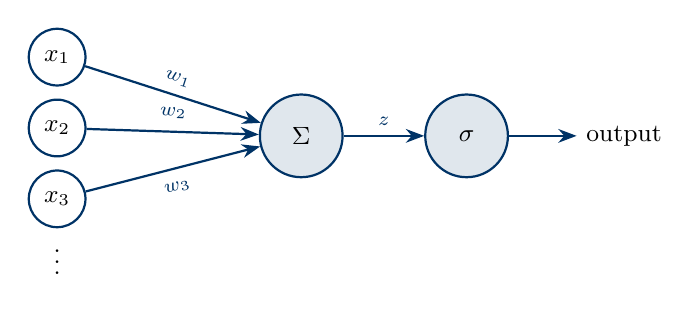
\begin{tikzpicture}[font=\small,
      inp/.style={circle, draw=sghblue, thick, minimum size=0.72cm},
      nrn/.style={circle, draw=sghblue, fill=sghblue!12, thick,
                  minimum size=1.05cm}]
    \node[inp] (x1) at (0, 1.4) {$x_1$};
    \node[inp] (x2) at (0, 0.5) {$x_2$};
    \node[inp] (x3) at (0, -0.4) {$x_3$};
    \node at (0, -1.1) {$\vdots$};
    \node[nrn] (s) at (3.1, 0.4) {$\Sigma$};
    \node[nrn] (a) at (5.2, 0.4) {$\sigma$};
    \node (out) at (7.2, 0.4) {output};
    \draw[-{Stealth}, thick, sghblue] (x1) -- node[above, sloped]
      {\scriptsize $w_1$} (s);
    \draw[-{Stealth}, thick, sghblue] (x2) -- node[above=1pt, sloped]
      {\scriptsize $w_2$} (s);
    \draw[-{Stealth}, thick, sghblue] (x3) -- node[below=1pt, sloped]
      {\scriptsize $w_3$} (s);
    \draw[-{Stealth}, thick, sghblue] (s) -- node[above]
      {\scriptsize $z$} (a);
    \draw[-{Stealth}, thick, sghblue] (a) -- (out);
  \end{tikzpicture}
  \end{center}
  \vspace{0.3em}
  \begin{itemize}\small
    \item Weighted sum, squashed: $\sigma(w_0 + w_1 x_1 + \dots)$.
          \alert{You met this in Block 2} - one neuron with a sigmoid
          \emph{is} logistic regression.
    \item Everything that follows is a strategy for wiring many of these
          together.
  \end{itemize}
\end{frame}

% ---------------------------------------------------------------
\begin{frame}{Stack and repeat: the multilayer perceptron}
  \begin{center}
  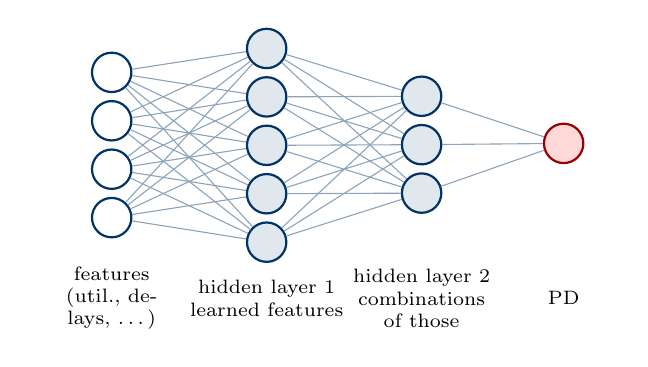
\begin{tikzpicture}[font=\scriptsize, scale=0.82,
      nd/.style={circle, draw=sghblue, thick, minimum size=0.5cm,
                 inner sep=1pt}]
    \foreach \i in {1,...,4} \node[nd] (i\i) at (0, -\i*0.75) {};
    \foreach \i in {1,...,5} \node[nd, fill=sghblue!12] (h\i)
      at (2.4, -\i*0.75+0.37) {};
    \foreach \i in {1,...,3} \node[nd, fill=sghblue!12] (g\i)
      at (4.8, -\i*0.75-0.37) {};
    \node[nd, fill=red!15, draw=red!60!black] (o) at (7.0, -1.85) {};
    \foreach \i in {1,...,4} \foreach \j in {1,...,5}
      \draw[sghblue!45, thin] (i\i) -- (h\j);
    \foreach \i in {1,...,5} \foreach \j in {1,...,3}
      \draw[sghblue!45, thin] (h\i) -- (g\j);
    \foreach \i in {1,...,3} \draw[sghblue!45, thin] (g\i) -- (o);
    \node[align=center, text width=1.9cm] at (0, -4.25)
      {features\\(util., delays, \ldots)};
    \node[align=center, text width=2.0cm] at (2.4, -4.25)
      {hidden layer 1\\\alert{learned features}};
    \node[align=center, text width=2.1cm] at (4.8, -4.25)
      {hidden layer 2\\combinations of those};
    \node[align=center, text width=1.2cm] at (7.0, -4.25) {PD};
  \end{tikzpicture}
  \end{center}
  \begin{itemize}\small
    \item Each hidden unit computes its own little logistic-like score of
          the layer below; the next layer combines \emph{those}.
    \item The network \alert{engineers its own features} - Block 1's
          craft, automated. That is the entire selling point.
  \end{itemize}
\end{frame}

% ---------------------------------------------------------------
\begin{frame}{Why depth at all: the XOR lesson}
  \begin{itemize}
    \item A single neuron is a linear cut - and famously \alert{cannot
          learn XOR} (``either-or''): no line separates the diagonal
          corners. That 1969 observation helped freeze the field for a
          decade.
    \item One hidden layer fixes it: two units each draw a line, the
          output combines them - the network builds
          \emph{either-side-of-both} as a \alert{learned feature}.
    \item Credit translation: ``risky iff \emph{high utilisation} XOR
          \emph{has savings buffer}'' - patterns whose pieces are
          individually uninformative. Trees find these too (B3);
          linear models need them hand-fed (B2's interactions).
  \end{itemize}
  \vspace{0.4em}
  \begin{center}\small
    Theory footnote: one wide-enough hidden layer can approximate any
    reasonable function - \emph{can} in principle, not \emph{will} from
    finite data. The U-curve is not repealed.
  \end{center}
\end{frame}

% ---------------------------------------------------------------
\begin{frame}{Counting the knobs (worked example)}
  Our lab network on 10 features: layers $10 \to 32 \to 16 \to 1$.
  \begin{center}\small
  \begin{tabular}{@{}lcc@{}}
    \toprule
    Layer & weights & biases \\
    \midrule
    input $\to$ hidden 1 & $10 \times 32 = 320$ & 32 \\
    hidden 1 $\to$ hidden 2 & $32 \times 16 = 512$ & 16 \\
    hidden 2 $\to$ output & $16 \times 1 = 16$ & 1 \\
    \midrule
    total & \multicolumn{2}{c}{\alert{897 parameters}} \\
    \bottomrule
  \end{tabular}
  \end{center}
  \vspace{0.4em}
  \begin{itemize}\small
    \item Logistic regression solved the same task with \alert{11}.
          On our 21{,}000 training rows, 897 knobs are comfortable -
          the same count on Block 1's little 2{,}800-row world needed a
          much tighter leash. Size the leash to the data.
    \item Modern LLMs: the same counting exercise, with $\sim$$10^{11}$
          knobs - and correspondingly astronomical data appetites.
  \end{itemize}
\end{frame}

% ---------------------------------------------------------------
\begin{frame}{Activations: the bend between the layers}
  \begin{center}
    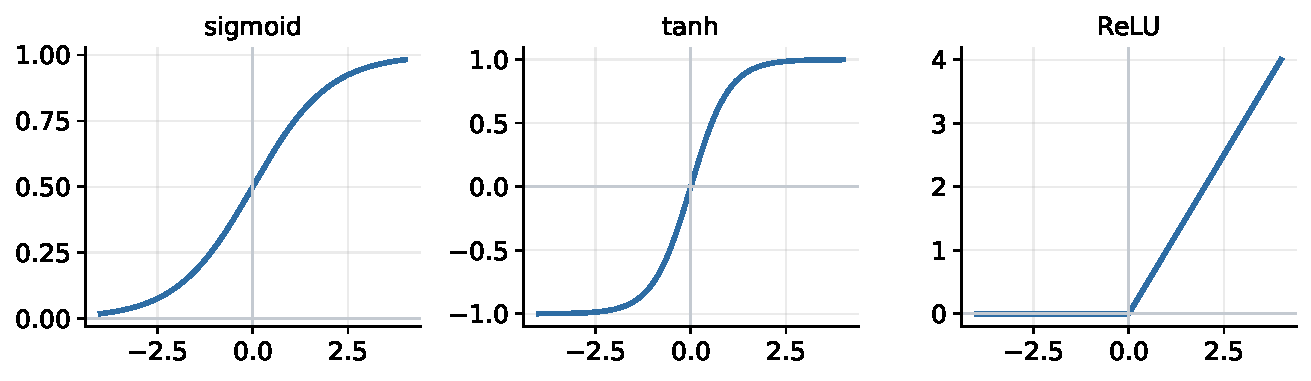
\includegraphics[width=0.88\textwidth]{figures/fig_activations.pdf}
  \end{center}
  \begin{itemize}\small
    \item Without a nonlinearity, stacked layers collapse into one big
          linear model - \alert{the bend is where the power lives}.
    \item Modern default: \textbf{ReLU} ($\max(0, z)$) - cheap, and its
          gradient doesn't vanish for large inputs the way sigmoid's does.
          Sigmoid survives at the \emph{output}, where we need a
          probability (Block 2 says hello).
  \end{itemize}
\end{frame}

% ---------------------------------------------------------------
\begin{frame}{Training: backpropagation without the tears}
  \begin{enumerate}
    \item \textbf{Forward}: push a batch of customers through; get
          predicted PDs.
    \item \textbf{Loss}: score them with \alert{log-loss} - the very
          same loss as logistic regression (Block 2, again).
    \item \textbf{Backward}: the chain rule attributes a share of the
          error to \emph{every weight} - that attribution is
          backpropagation, and it is bookkeeping, not magic.
    \item \textbf{Step}: nudge each weight downhill a little
          (\alert{gradient descent}); repeat for many epochs:
          \[
            w \;\leftarrow\; w - \eta \, \frac{\partial L}{\partial w}
            \qquad (\eta = \text{learning rate})
          \]
  \end{enumerate}
  \vspace{0.5em}
  \begin{center}\small
    Unlike OLS there is no closed form and unlike logistic regression the
    landscape isn't convex - many valleys, so \alert{initialisation and
    seeds matter} (reproducibility rule, weights edition).
  \end{center}
\end{frame}

% ---------------------------------------------------------------
\begin{frame}{Stochastic gradient descent: learning in batches}
  \begin{itemize}
    \item Computing the exact gradient means touching \emph{every}
          customer per step - accurate, slow, and pointless at scale.
    \item \textbf{SGD}: estimate the gradient on a random
          \alert{mini-batch} (say 200 customers), step, repeat. One pass
          through all batches = one \alert{epoch}.
    \item Noisy steps are a feature: the jitter helps escape bad valleys
          of the non-convex landscape - controlled chaos, like
          bootstrap's controlled resampling (B3).
    \item \textbf{Adam} (the default optimiser) adds per-weight adaptive
          step sizes and momentum - fewer tantrums, \alert{but it is
          still gradient descent with a learning rate} you own.
  \end{itemize}
\end{frame}

% ---------------------------------------------------------------
\begin{frame}{Output layers: one task, one head}
  \small
  \begin{center}
  \begin{tabular}{@{}llll@{}}
    \toprule
    Task & Output layer & Loss & Course tie \\
    \midrule
    Binary PD & 1 unit, sigmoid & log-loss & Blocks 2--3 \\
    Multiclass routing & 5 units, \alert{softmax} & cross-entropy & Block 5 \\
    Regression (LGD) & 1 unit, linear & squared error & Block 2 \\
    \bottomrule
  \end{tabular}
  \end{center}
  \vspace{0.5em}
  \begin{itemize}\small
    \item Softmax = the multi-way sigmoid: five scores in, five
          probabilities out, summing to one - the complaint router's
          native output head:
          $\;p_k = e^{z_k} \big/ \sum_j e^{z_j}$.
    \item The body of the network is task-agnostic feature machinery;
          \alert{only the head and the loss change}. That one design idea
          carries all of deep learning.
    \item It also means one body can serve \emph{several} heads at once
          (PD and LGD from shared learned features) - multi-task
          learning, mentioned so the term has a home.
  \end{itemize}
\end{frame}

% ---------------------------------------------------------------
\begin{frame}{What the bend buys: moons, revisited}
  \begin{center}
    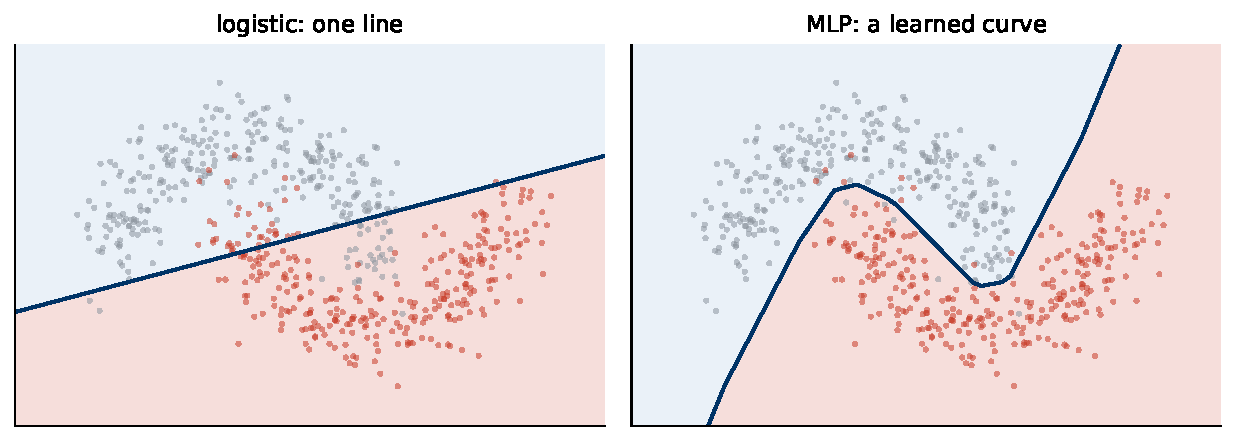
\includegraphics[width=0.86\textwidth]{figures/fig_mlp_boundary.pdf}
  \end{center}
  \begin{itemize}\small
    \item Block 3's crescents, third visit: logistic must draw a line;
          the MLP \alert{learns the curve} - no hand-engineered
          features, no axis-aligned rectangles.
    \item Smooth learned boundaries are the MLP's signature - compare
          the tree's staircase.
  \end{itemize}
\end{frame}

% ---------------------------------------------------------------
\begin{frame}{Capacity: the U-curve, neural edition}
  \begin{center}
    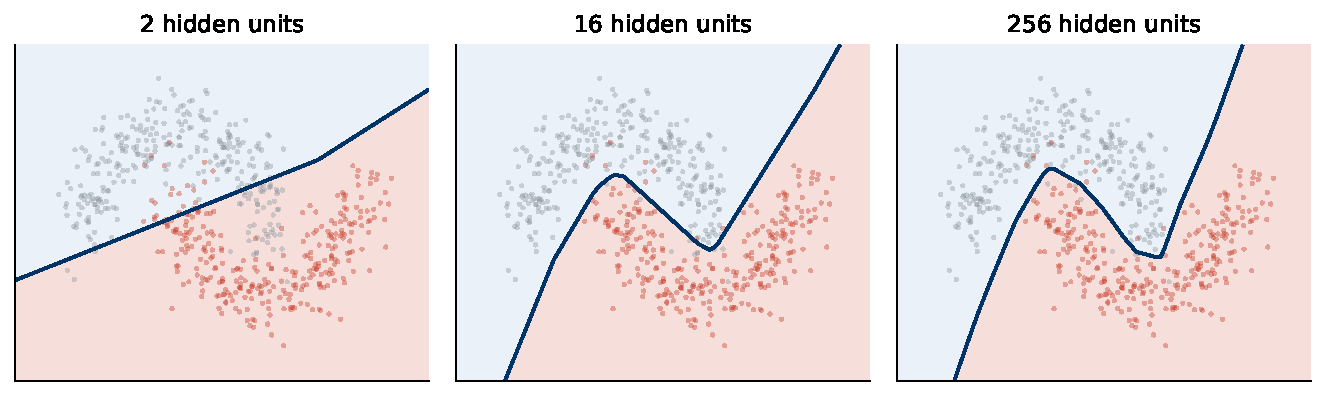
\includegraphics[width=0.9\textwidth]{figures/fig_capacity.pdf}
  \end{center}
  \begin{itemize}\small
    \item Two hidden units underfit; 256 memorise the noise along the
          edge. \alert{Width and depth are the capacity dials.}
    \item You knew this was coming: same U-curve as polynomial degree,
          tree depth, and $1/\alpha$. Nothing about neural networks
          repeals Block 2.
  \end{itemize}
\end{frame}

% ============================================================
% SECTION: TRAINING
% ============================================================
\section{Training}

% ---------------------------------------------------------------
\begin{frame}{Watching a network learn}
  \begin{center}
    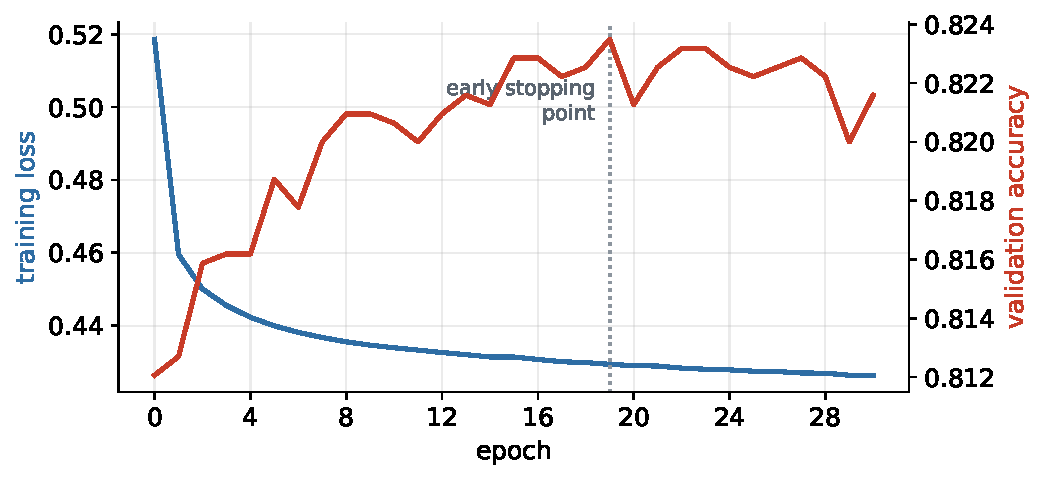
\includegraphics[width=0.7\textwidth]{figures/fig_loss_curve.pdf}
  \end{center}
  \begin{itemize}\small
    \item Training loss falls forever; \alert{validation accuracy} rises,
          peaks, and decays as memorisation sets in - \textbf{early
          stopping} halts training at the peak: the network's everyday
          leash.
    \item This one plot is your first diagnostic for any training run -
          learn to read it before you learn any architecture.
  \end{itemize}
\end{frame}

% ---------------------------------------------------------------
\begin{frame}{The learning rate: one knob to rule your evening}
  \begin{center}
    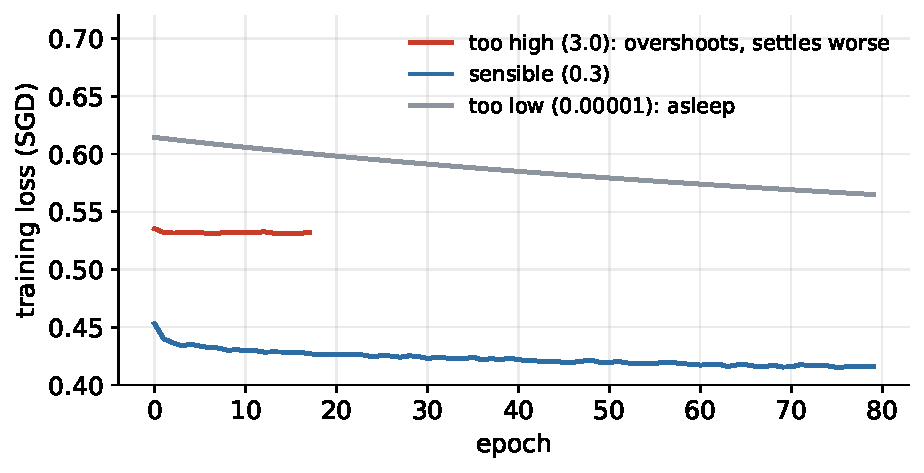
\includegraphics[width=0.66\textwidth]{figures/fig_lr_effect.pdf}
  \end{center}
  \begin{itemize}\small
    \item Too high: the steps overshoot the narrow valley and settle at a
          \alert{worse} loss. Too low: the network is asleep. The usable
          band spans \alert{orders of magnitude} - search it on a log
          scale (Block 3's tuning advice applies).
    \item GBDT's learning rate is the same concept - humble steps,
          more of them.
  \end{itemize}
\end{frame}

% ---------------------------------------------------------------
\begin{frame}{The leash inventory (where is its leash? - answered)}
  \small
  \begin{center}
  \begin{tabular}{@{}lll@{}}
    \toprule
    Leash & Mechanism & Course cousin \\
    \midrule
    Early stopping & stop at the validation plateau & GBDT rounds (B3) \\
    Weight decay (L2) & penalise large weights & ridge (B2) \\
    Dropout & randomly silence units while training & bagging-ish (B3) \\
    Smaller network & fewer units/layers & tree depth (B3) \\
    More data & the only leash that adds signal & - everyone's \\
    \bottomrule
  \end{tabular}
  \end{center}
  \vspace{0.5em}
  \begin{itemize}\small
    \item Every mechanism is new; \alert{no idea is new}. Ask the fixed
          question - where is the leash? - and any future architecture
          becomes familiar in an afternoon.
  \end{itemize}
\end{frame}

% ---------------------------------------------------------------
\begin{frame}{Practicalities that bite}
  \begin{itemize}
    \item \textbf{Scale your features} - gradient descent on unscaled
          inputs limps; the pipeline with \texttt{StandardScaler} is
          mandatory again (penalties country, not trees country).
    \item \textbf{Seeds}: random initialisation $\Rightarrow$ different
          runs, different networks; fix \texttt{random\_state}, expect
          run-to-run wobble anyway.
    \item \textbf{Missing values}: no native handling - back to Block 1's
          impute-plus-indicator. (GBDT stays more convenient here.)
    \item \textbf{Cost}: minutes-not-milliseconds training, more tuning
          surface, hungrier for data - all of it must be \alert{paid for
          by accuracy} we can measure.
  \end{itemize}
  \vspace{0.4em}
  \begin{center}\small
    sklearn's \texttt{MLPClassifier} is enough for foundations; industry
    reaches for PyTorch when architectures get custom.
  \end{center}
\end{frame}

% ---------------------------------------------------------------
\begin{frame}{Debugging a training run (field checklist)}
  \begin{enumerate}
    \item \textbf{Loss is NaN / exploding} $\to$ learning rate too high;
          drop it 10$\times$.
    \item \textbf{Loss flat from epoch one} $\to$ rate too low, features
          unscaled, or a dead ReLU layer.
    \item \textbf{Train great, validation ugly} $\to$ the U-curve says
          hello: tighten a leash (early stopping, decay, width).
    \item \textbf{Can it overfit 100 rows?} - the classic smoke test: a
          healthy network memorises a tiny sample \alert{perfectly}; if
          it cannot, the bug is in your pipeline, not your patience.
    \item \textbf{Run twice} - seed wobble bigger than your claimed
          improvement means you claimed noise (CV spread, B3).
  \end{enumerate}
  \vspace{0.3em}
  \begin{center}\small
    Note the shape of this list: it is Block 1's read-the-traceback
    discipline, upgraded to a stochastic system.
  \end{center}
\end{frame}

% ============================================================
% SECTION: VERDICT
% ============================================================
\section{Verdict}

% ---------------------------------------------------------------
\begin{frame}{The final tournament}
  \begin{center}
    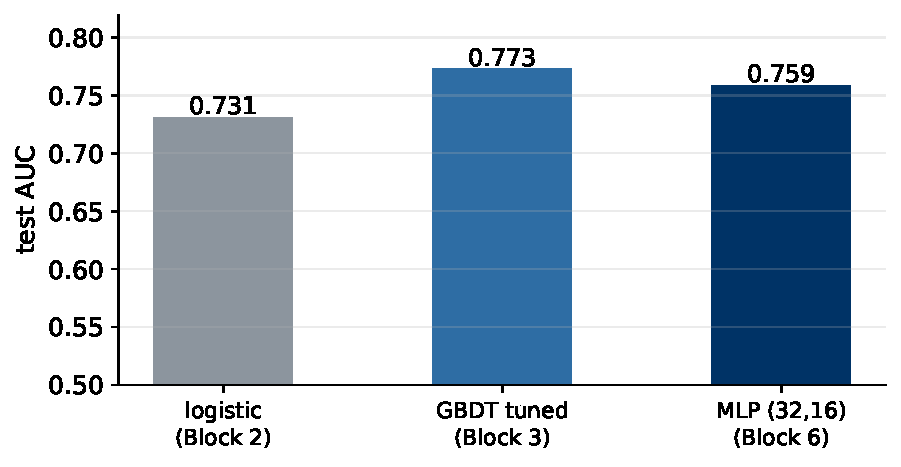
\includegraphics[width=0.6\textwidth]{figures/fig_final_tournament.pdf}
  \end{center}
  \begin{itemize}\small
    \item MLP: \alert{0.759} - clears the baseline by $+2.8$ points
          (complexity \alert{earned}) yet still trails the tuned GBDT
          (0.773).
    \item So the real portfolio's final order: GBDT $>$ MLP $>$ SVM
          $\approx$ logistic. The most fashionable family takes
          \alert{second place} - the tabular crown stays with boosted
          trees, exactly what the benchmark literature predicts.
  \end{itemize}
\end{frame}

% ---------------------------------------------------------------
\begin{frame}{When do neural networks actually win?}
  \begin{itemize}
    \item \textbf{Perception \& sequence data} - images, speech, text,
          time series: layers exploit \alert{structure} (pixels near
          pixels, words after words) that tabular rows simply lack.
    \item \textbf{Huge tabular data with interactions} - millions of
          rows, thousands of features: sometimes; benchmark studies still
          crown \alert{GBDT} on most mid-size tabular problems.
    \item \textbf{Entity embeddings} - thousands-of-category features
          (merchant IDs) learned into dense vectors: a genuine tabular
          win, and the same idea behind Block 5's word embeddings.
    \item \textbf{Representation reuse} - autoencoders (Block 4's
          reconstruction lens, nonlinear edition), pretrained models,
          transfer.
  \end{itemize}
  \vspace{0.3em}
  \begin{center}\small
    Rule of the shop, final form: logistic $\to$ GBDT $\to$ deep, each
    step only \alert{after} the previous one is beaten on honest numbers.
  \end{center}
\end{frame}

% ---------------------------------------------------------------
\begin{frame}{What we skipped on purpose (and where it lives)}
  \begin{itemize}
    \item \textbf{CNNs} - convolutions exploit ``pixels near pixels'';
          vision's workhorse.
    \item \textbf{RNNs $\to$ Transformers} - sequence models; attention
          (2017) is why LLMs exist. Block 2's ``why these models'' slide
          and this table are cousins, not rivals.
    \item \textbf{Autoencoders} - Block 4's compress-and-reconstruct
          lens, nonlinear; used for anomaly scores (reconstruction error
          on a weird customer is high).
    \item \textbf{Pretraining \& transfer} - borrow representations
          learned elsewhere; the economics behind embedding APIs (B5).
  \end{itemize}
  \vspace{0.4em}
  \begin{center}\small
    Foundations were the deliverable: with the neuron, the loss, SGD and
    the leash inventory, each of these is one focused week of reading -
    not a new religion.
  \end{center}
\end{frame}

% ---------------------------------------------------------------
\begin{frame}{The interpretability bill}
  \begin{itemize}
    \item Block 2's receipt was \alert{exact and free}. Trees gave a path.
          The MLP's weights are thousands of numbers with \alert{no
          individual meaning} - explanation becomes reconstruction
          (SHAP and friends), approximate and costly.
    \item In regulated lending the bill is concrete: adverse-action
          reasons, model validation teams, regulator Q\&A - each harder,
          slower, more contestable.
    \item So the trade is not ``accuracy vs beauty''; it is accuracy vs
          \alert{auditability, monitoring cost, and legal risk} - priced
          per use case.
  \end{itemize}
  \vspace{0.5em}
  \begin{center}
    A 0.5-point AUC gain that costs your explanation is a bad trade at a
    bank and a fine trade in ad-click ranking. \alert{Context prices it.}
  \end{center}
\end{frame}

% ---------------------------------------------------------------
\begin{frame}{Choosing the model family: the course's one table}
  \footnotesize
  \begin{center}
  \begin{tabular}{@{}llllll@{}}
    \toprule
     & logistic & tree & SVM & GBDT/RF & MLP \\
    \midrule
    Interactions & by hand & native & kernel & native & native \\
    Scaling needed & yes & no & yes & no & yes \\
    Missing values & impute+flag & impute & impute & native (Hist) & impute+flag \\
    Explanation & exact receipt & the path & hard & SHAP approx. & SHAP approx. \\
    Probabilities & native & chunky & calibrate & good & native \\
    Tuning burden & tiny & small & moderate & moderate & \alert{large} \\
    Small data & \alert{strong} & weak & good & good & weak \\
    Typical tabular rank & baseline & - & mid & \alert{top} & varies \\
    Regulator comfort & \alert{high} & high & low & moderate & low \\
    \bottomrule
  \end{tabular}
  \end{center}
  \vspace{0.4em}
  \begin{center}\small
    Print this one. Every ``which model should we use?'' meeting is this
    table plus costs.
  \end{center}
\end{frame}

% ============================================================
% SECTION: RESPONSIBLE ML
% ============================================================
\section{Responsible ML}

% ---------------------------------------------------------------
\begin{frame}{Why this section exists}
  \begin{itemize}
    \item A wrong sales forecast wastes money. A wrong \alert{credit
          model} declines the wrong people, systematically, at scale,
          silently - the social consequences the course outcomes
          (K3) name explicitly.
    \item Every earlier block planted a piece: selection bias (B1),
          probabilities that price people (B2--3), segments that must not
          decide (B4), PII in text (B5).
    \item This section assembles them - on \alert{our own model's
          numbers}, not hypotheticals.
  \end{itemize}
  \vspace{0.5em}
  \begin{center}
    The operating question is never ``is the model accurate?'' -
    it is \alert{``what does the model do to people, and who checked?''}
  \end{center}
\end{frame}

% ---------------------------------------------------------------
\begin{frame}{The legal floor (EU, sketched)}
  \begin{itemize}
    \item \textbf{GDPR Art.\ 22}: individuals may not be subject to purely
          automated decisions with legal effect - credit is the textbook
          case - without safeguards: \alert{human review on request,
          meaningful information about the logic}.
    \item \textbf{Duty to state reasons}: declined customers are informed
          of the grounds - true ones (Block 1's punchline was never just
          about imputation hygiene; the US calls this ``adverse action'').
    \item \textbf{Protected attributes}: sex, ethnicity, and friends
          are off-limits for credit decisions - which is precisely why we
          audit \alert{by sex} on the next slides; age sits in a grey,
          jurisdiction-dependent zone (lab exercise).
    \item \textbf{EU AI Act}: credit scoring is listed \alert{high-risk}
          - documentation, monitoring, human oversight become statutory,
          not best-practice.
  \end{itemize}
  \vspace{0.3em}
  \begin{center}\small
    Sketch, not legal advice - the real thing is done \alert{with
    lawyers in the room}. Your job is to know when to invite them: earlier
    than feels natural.
  \end{center}
\end{frame}

% ---------------------------------------------------------------
\begin{frame}{Where bias enters the pipeline}
  \small
  \begin{center}
  \begin{tabular}{@{}lp{5.2cm}l@{}}
    \toprule
    Door & Mechanism & Course tie \\
    \midrule
    Labels & ``default'' reflects \emph{past} collection practices & B1 \\
    Selection & approved-only data; the rejected are absent & B1 \\
    Features & proxies encode group membership & today \\
    Measurement & income verified differently across segments & B1 \\
    Objective & optimising average cost ignores who pays it & B3 \\
    Feedback & the model's own decisions write next year's data & next slide \\
    \bottomrule
  \end{tabular}
  \end{center}
  \vspace{0.5em}
  \begin{center}
    None of these doors is opened by malice. All of them are opened by
    \alert{default}, unless someone checks.
  \end{center}
\end{frame}

% ---------------------------------------------------------------
\begin{frame}{Feedback loops: the model writes its own future data}
  \begin{itemize}
    \item Decline a group more often $\Rightarrow$ fewer loans observed
          $\Rightarrow$ \alert{no evidence the declines were wrong}
          $\Rightarrow$ next year's model, trained on the new data,
          declines them again - with better ``justification''.
    \item This is Block 1's selection bias, \alert{motorised}: the model
          doesn't just inherit the bias, it manufactures more of it.
    \item Breakers: reject inference (B1's vocabulary), deliberate
          exploration (approve a small random slice near the boundary -
          expensive, informative), and monitoring group gaps over
          \emph{vintages}, not snapshots.
    \item Any system that acts on its own predictions has one of these
          loops. Finding it is part of the job now.
  \end{itemize}
\end{frame}

% ---------------------------------------------------------------
\begin{frame}{Fairness has competing definitions}
  For a protected group $g$ and decisions $\hat{y}$:
  \small
  \begin{center}
  \begin{tabular}{@{}lll@{}}
    \toprule
    Criterion & Demands equal\ldots & In credit terms \\
    \midrule
    Demographic parity & $P(\hat{y}{=}1 \mid g)$ & decline rates \\
    Equalised odds & FPR and FNR per group & wrongly-declined \& missed rates \\
    Calibration by group & $P(y{=}1 \mid \hat{p}, g)$ & a 0.3 means 0.3 for everyone \\
    \bottomrule
  \end{tabular}
  \end{center}
  \vspace{0.5em}
  \begin{itemize}\small
    \item All three sound obviously right. \alert{Mathematically, they
          cannot hold at once} when base rates differ between groups
          (Kleinberg et al., Chouldechova, 2016--17).
    \item So ``make it fair'' is not a specification - \emph{choosing
          which fairness} is the decision, and it is not the data
          scientist's alone.
  \end{itemize}
\end{frame}

% ---------------------------------------------------------------
\begin{frame}{Our own model, audited by sex}
  \begin{center}
    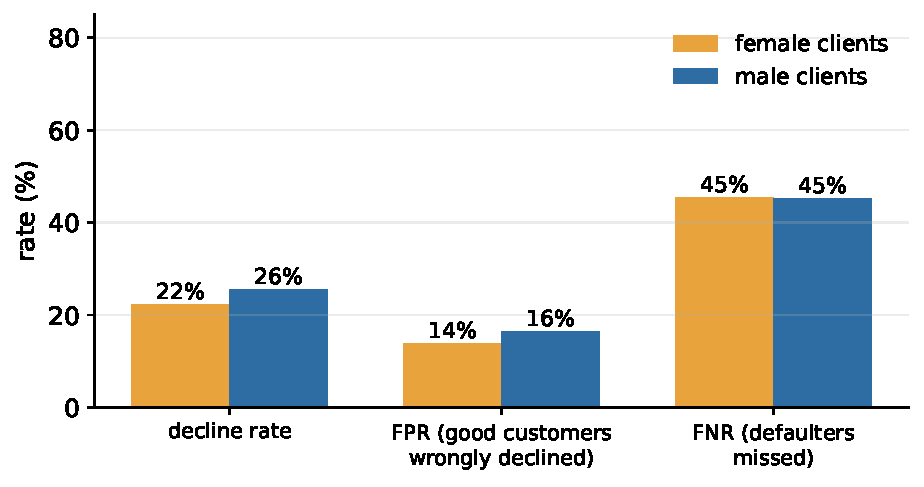
\includegraphics[width=0.58\textwidth]{figures/fig_fairness.pdf}
  \end{center}
  \begin{itemize}\small
    \item GBDT at Block 3's cost-optimal threshold: men declined at
          \alert{25.6\% vs 22.3\%} for women, FPR \alert{16.5\% vs
          13.8\%} - with base default rates of 23.9\% vs 21.0\%.
    \item Read honestly: the gaps are \alert{modest and track the
          base-rate difference} - this model does not amplify. (It can
          go the other way: on Block 1's synthetic portfolio, an age audit
          turned a 3.6 pp base gap into an 18 pp decline gap.) You only
          know \alert{after} you measure - which is the point.
  \end{itemize}
\end{frame}

% ---------------------------------------------------------------
\begin{frame}{``Just remove sex'': the unawareness experiment}
  \begin{center}
    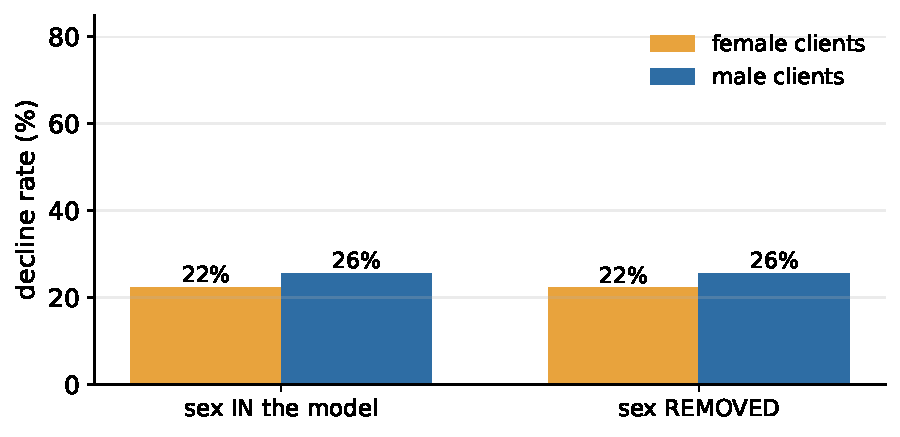
\includegraphics[width=0.56\textwidth]{figures/fig_proxy.pdf}
  \end{center}
  \begin{itemize}\small
    \item Removal changes \alert{essentially nothing}: every bar is
          identical with or without the column. The model never needed
          \texttt{sex} - six months of payment behaviour already carries
          whatever group structure exists. That is \alert{proxy
          discrimination} stated at its purest: deleting the label does not
          delete the information.
    \item Corollary: ``fairness through unawareness'' here is free -
          and toothless. If the measured gaps needed fixing, the fix would
          have to act on \alert{decisions} (thresholds, constraints), not
          on the column list.
  \end{itemize}
\end{frame}

% ---------------------------------------------------------------
\begin{frame}{The mitigation menu (survey level)}
  \begin{itemize}
    \item \textbf{Pre-processing}: fix the data - rebalance, collect
          better labels (recall selection bias: the rejected are
          missing by construction). Removing proxies alone is the
          unawareness trap we just watched fail.
    \item \textbf{In-processing}: fairness constraints inside training
          (equalised-odds penalties; monotonic constraints were a mild
          cousin).
    \item \textbf{Post-processing}: per-group thresholds - effective,
          transparent, and \alert{legally delicate} (explicitly using the
          protected attribute to fix its own harm).
    \item Always available: \alert{measure and publish} the gaps
          internally, so the trade-off is decided by people entitled to
          decide it.
  \end{itemize}
  \vspace{0.4em}
  \begin{center}\small
    Toolkits exist (fairlearn, AIF360) - the hard part was never the
    code.
  \end{center}
\end{frame}

% ---------------------------------------------------------------
\begin{frame}{Responsibility beyond fairness}
  \begin{itemize}
    \item \textbf{Drift \& monitoring}: models rot as portfolios move
          (B3); yesterday's fair model can be today's unfair one -
          monitor \alert{gaps}, not just Gini.
    \item \textbf{Documentation}: features with time-travel audits (B3),
          imputation recipes (B1), threshold rationale (B3), fairness
          measurements (today) - if it isn't written down, it doesn't
          exist at audit time.
    \item \textbf{Human oversight}: confidence bars and human queues (B5)
          are not UX niceties; under the AI Act they are architecture.
    \item \textbf{Privacy}: PII in text (B5), data minimisation -
          collect what the decision needs, not what the crawler found.
  \end{itemize}
\end{frame}

% ---------------------------------------------------------------
\begin{frame}{Who decides: model governance in a bank}
  \begin{itemize}
    \item \textbf{First line} - you, the builder: measurements, docs,
          honesty clauses. Everything this course drilled.
    \item \textbf{Second line} - independent \alert{model validation}:
          rebuilds your results, attacks your assumptions; a good one is a
          professional adversarial verifier (and a common first job for
          this course's graduates).
    \item \textbf{Model risk committee} - owns the accept/reject and the
          trade-offs no analyst should carry alone (which fairness, whose
          cost).
    \item \textbf{Audit \& regulator} - arrive later, read everything;
          the written trail \emph{is} the model at that point.
  \end{itemize}
  \vspace{0.4em}
  \begin{center}\small
    The fairness-metric choice from four slides ago lands \alert{here} -
    with lawyers and the committee, informed by your measurements.
  \end{center}
\end{frame}

% ---------------------------------------------------------------
\begin{frame}{The responsible-ML checklist (take-home)}
  \begin{enumerate}
    \item Every feature: \emph{when is it known?} and \emph{may we use
          it?} - two written answers per column.
    \item Fairness gaps \alert{measured} (decline, FPR, FNR, calibration
          by group) before go-live and on schedule after.
    \item Explanation path exists for every declined customer - and it
          is \alert{true}.
    \item A human can be reached, and can overrule.
    \item Monitoring alarms on drift \emph{and} on gap widening.
    \item The model's owner is a name, not a department.
  \end{enumerate}
  \vspace{0.4em}
  \begin{center}\small
    Six lines; most model-risk findings in the wild are a missing line
    from this list.
  \end{center}
\end{frame}

% ============================================================
% SECTION: BRIEFING
% ============================================================
\section{Briefing}

% ---------------------------------------------------------------
\begin{frame}{Next week: how the presentation works}
  \begin{itemize}
    \item \alert{$\sim$6--8 minutes per team} + questions: business framing
          $\to$ data work $\to$ two model families vs a baseline $\to$
          honest evaluation $\to$ recommendation.
    \item \alert{Upload deadline: before Block 7 starts} - all code (a
          reproducible notebook) \emph{and} the exact presentation you will
          show. We may run your notebook top to bottom (Restart \& Run All
          has been the habit since Block 1 - this is why).
    \item \textbf{The AI rule}: assistants were allowed all semester, but
          you answer for every submitted line. The more the project feels
          written \emph{solely} by AI, the \alert{harder the questions} -
          expect to explain and modify your code live.
    \item Bring the \alert{honesty kit}: CV spread, leakage audit,
          threshold argument, limitations paragraph.
  \end{itemize}
  \vspace{0.3em}
  \begin{center}\small
    Rubric weights, one more time: framing 10 / data prep 15 / modelling
    15 / evaluation 20 / interpretation 15 / reproducibility 5 /
    \alert{presentation \& defence 20}.
  \end{center}
\end{frame}

% ---------------------------------------------------------------
\begin{frame}{Defence failure modes (from the graveyard)}
  \begin{enumerate}
    \item A suspiciously high AUC presented \alert{proudly} (you know the
          smell now - find the leak before we do).
    \item Accuracy on an imbalanced target, unexamined.
    \item Complex model, no baseline - ``earned its keep'' cannot be
          claimed without the keeper.
    \item Segments/rules with no honesty clause (silhouette, lift vs
          confidence).
    \item A notebook that only runs in the order it was written in -
          which is to say, doesn't.
    \item Recommendation missing: analysis that ends in metrics instead of
          \alert{a decision}.
  \end{enumerate}
\end{frame}

% ---------------------------------------------------------------
\begin{frame}{The exam (term 0): what to expect}
  \begin{itemize}
    \item Second half of Block 7, \alert{120 minutes}. \alert{$\sim$40\%}
          conceptual multiple choice; \alert{$\sim$60\%} short open
          questions: pick a method for a described problem, interpret a
          given output. One question from each block's practice slide
          appears on the paper - revision pays, literally.
    \item It tests \textbf{selection} and \textbf{interpretation} -
          W3/W4 - not derivations: expect ``here is a confusion matrix /
          rule / coefficient / dendrogram - what do you tell the
          business?''
    \item Worked-example slides (Gini split, silhouette, the rule
          arithmetic, odds ratios) are the calibration for the by-hand
          questions.
    \item Best study kit: the six \alert{``Block $N$ in five sentences''}
          slides - they are the syllabus, compressed.
  \end{itemize}
\end{frame}

% ============================================================
% SECTION: LAB
% ============================================================
\section{Lab}

% ---------------------------------------------------------------
\begin{frame}[plain]
  \begin{center}
    \vspace{1.5cm}
    {\LARGE\textbf{Laboratory}}\\[0.6cm]
    {\normalsize Notebook \texttt{06\_neural\_networks} - laptops out.}
  \end{center}
\end{frame}

% ---------------------------------------------------------------
\begin{frame}{Lab today}
  \begin{columns}[T]
    \begin{column}{0.54\textwidth}
      \textbf{Notebook \texttt{06\_neural\_networks}}
      \begin{itemize}\small
        \item train an MLP on the PD task, in a pipeline
        \item read its loss curve; move the learning rate
        \item run the final tournament yourselves
        \item audit the model by sex - then by age (exercise) -
              and try the removal experiment
      \end{itemize}
    \end{column}
    \begin{column}{0.44\textwidth}
      \textbf{Project questions welcome}
      \begin{itemize}\small
        \item last chance to ask in person before the presentation
        \item stuck on something? ask \alert{today}, not the night
              before the upload
      \end{itemize}
    \end{column}
  \end{columns}
  \vspace{0.5em}
  \begin{center}\small
    ``Done'' = your MLP verdict matches your tournament table, and your
    fairness audit has numbers in it.
  \end{center}
\end{frame}

% ============================================================
% SECTION: SUMMARY
% ============================================================
\section{Summary}

% ---------------------------------------------------------------
\begin{frame}[plain]
  \begin{center}
    \vspace{1.5cm}
    {\LARGE\textbf{Summary}}\\[0.6cm]
    {\normalsize What to take home - from the block, and the course.}
  \end{center}
\end{frame}

% ---------------------------------------------------------------
\begin{frame}{The course in five sentences}
  \begin{enumerate}
    \item Start from the \textbf{decision}; translate it into a task; look
          at the data before any model touches it.
    \item Judge everything on \textbf{unseen data}, with the right metric
          for the question and money attached to the threshold.
    \item Every model family has a \textbf{leash}, and complexity must
          \textbf{earn its keep} against a baseline - on real data it
          did, and the baseline was how we measured by how much.
    \item Structure without labels is found, argued and \textbf{named} -
          honestly, with a noise check.
    \item Models act on people: \textbf{explanations, fairness gaps and
          human oversight} are deliverables, not decoration.
  \end{enumerate}
  \vspace{0.5em}
  \begin{center}
    The subtitle kept its promise: \alert{how not to fool yourself.}
  \end{center}
\end{frame}

% ---------------------------------------------------------------
\begin{frame}{Project status \& reminder: the night before the defence}
  \begin{enumerate}
    \item \alert{Upload everything before class}: all code + the exact
          presentation. What you upload is what you present.
    \item \textbf{Restart \& Run All} - on a machine that isn't yours if
          you can.
    \item Every number on your slides \alert{traceable} to a notebook
          cell.
    \item One sentence ready per rubric row - especially
          \emph{interpretation}: what should the business \emph{do}?
    \item The two questions you fear most - written down, with your best
          honest answers (``we didn't have time to X'' beats improvised
          fiction).
    \item Timing: 6--8 minutes is \alert{$\sim$6 slides of content}, not 20.
          Rehearse once, aloud.
    \item Sleep. A rested ``I don't know, but here's how I'd find out''
          outscores a tired bluff every time.
  \end{enumerate}
\end{frame}

% ---------------------------------------------------------------
\begin{frame}{Exam practice - multiple choice}
  \small
  \textbf{Q1.} The role of early stopping when training an MLP:
  \begin{enumerate}[(a)]
    \item it speeds up each epoch
    \item it watches a validation score and halts training before the
          network overfits - the network's everyday leash
    \item it prevents exploding gradients
    \item it reduces the parameter count
  \end{enumerate}
  \vspace{0.4em}
  \textbf{Q2.} Removing \texttt{sex} from the features left every fairness
  metric essentially unchanged. Why?
  \begin{enumerate}[(a)]
    \item the audit code was broken
    \item the model was already fair, so nothing could change
    \item other features carry (proxy) the same group information -
          deleting the label does not delete the information
    \item sex was never predictive to begin with
  \end{enumerate}
\end{frame}
% Answer key: Q1 (b) - same U-curve control as max_depth for trees and C for
% logistic. Q2 (c) - proxy discrimination; "fairness through unawareness"
% fails whenever behaviour correlates with the group, which is almost always.

% ---------------------------------------------------------------
\begin{frame}{Exam practice - open question}
  \begin{block}{In the style of the term-0 exam ($\sim$60\% open questions)}
    On the tabular PD task: logistic 0.731, MLP 0.759, GBDT 0.773 test AUC.
    Which model do you recommend deploying, and what \emph{besides} AUC
    belongs in that decision? Name at least three considerations.
  \end{block}
  \vspace{0.5em}
  \begin{center}\small
    4-6 sentences. W3 in its purest form: select and defend.
  \end{center}
\end{frame}
% A good answer: GBDT on the numbers - but the defence must weigh:
% calibration (pricing needs honest probabilities), interpretability and
% adverse-action reasons (regulated decisions), monotonicity/regulator
% comfort, fairness-audit results at the operating threshold, and the
% monitoring/retraining cost of each family. Extra credit for noting the
% logistic baseline remains the yardstick any complexity must keep beating.

% ---------------------------------------------------------------
\begin{frame}[plain]
  \begin{center}
    \vspace{1.5cm}
    {\LARGE\textbf{Next week: defences \& exam.}}\\[0.6cm]
    {\normalsize Bring the honesty kit. Good luck - you won't need it.}
  \end{center}
\end{frame}

% ---------------------------------------------------------------
\begin{frame}{Keep learning - Block 6 reading}
  \begin{itemize}
    \item \textbf{LeCun, Bengio \& Hinton} - \emph{Deep Learning} (Nature,
          2015) - the canonical review article; where today's foundations
          lead.
    \item \textbf{3Blue1Brown} - the neural-network video series: the best
          visual account of backpropagation available.
    \item \textbf{Barocas, Hardt \& Narayanan} - \emph{Fairness and Machine
          Learning} (free at fairmlbook.org) - today's fairness section,
          in full.
    \item \textbf{Rudin} - \emph{Stop Explaining Black Box Models for
          High Stakes Decisions...} (Nature Machine Intelligence, 2019) -
          the interpretability bill, argued sharply.
  \end{itemize}
\end{frame}

\end{document}
